\section{Техническое задание}
\subsection{Основание для разработки}


Основанием для разработки является задание на выпускную квалификационную работу бакалавра "<Интеллектуальная система распознавания и классификации возгораний, полученных с БПЛА">.

\subsection{Цель и назначение разработки}

Программно-информационная система предназначена для автоматизации процесса обнаружения и классификации возгораний, повышения эффективности мониторинга пожароопасных зон и поддержки принятия информированных решений при реагировании на потенциальные угрозы.

Посредством создания интеллектуальной системы мы стремимся революционизировать процесс обнаружения и реагирования на пожары, а также позволить специалистам быстро и эффективно определять возгорания без лишних затрат.

Задачами данной разработки являются:
\begin{itemize}
	\item создание информационной базы для выбора нескольких изображений для последовательной классификации;
	\item предоставление предварительной обработки изображения для распознавания;
	\item реализация классификации возгораний по типу;
	\item выявление оценки степени опасности возгорания;
	\item обучение нейронной сети на подготовленных данных;
	\item оптимизация параметров сети для достижения максимальной точности распознавания;
	\item создание удобного и эффективного пользовтельского интерфейса.
\end{itemize}

\subsection{Требования пользователя к интерфейсу приложения}

Приложение должно включать в себя:
\begin{itemize}
    \item графический интерфейс пользователя;
    \item возможность загрузки изображений с БПЛА для их распознавания;
    \item отображение результата распознавания с указанием класса возгорания и степень опасности, а также уверенность в распознавании;
    \item возможность загрузки данных обучения для улучшения качества распознавания;
    \item возможность вывода полученных изображений с распознанным возгоранием для дальнейшего использования.
\end{itemize}

Композиция шаблона программы представлена на рисунке ~\ref{shablon:image}.

\begin{figure}[ht]
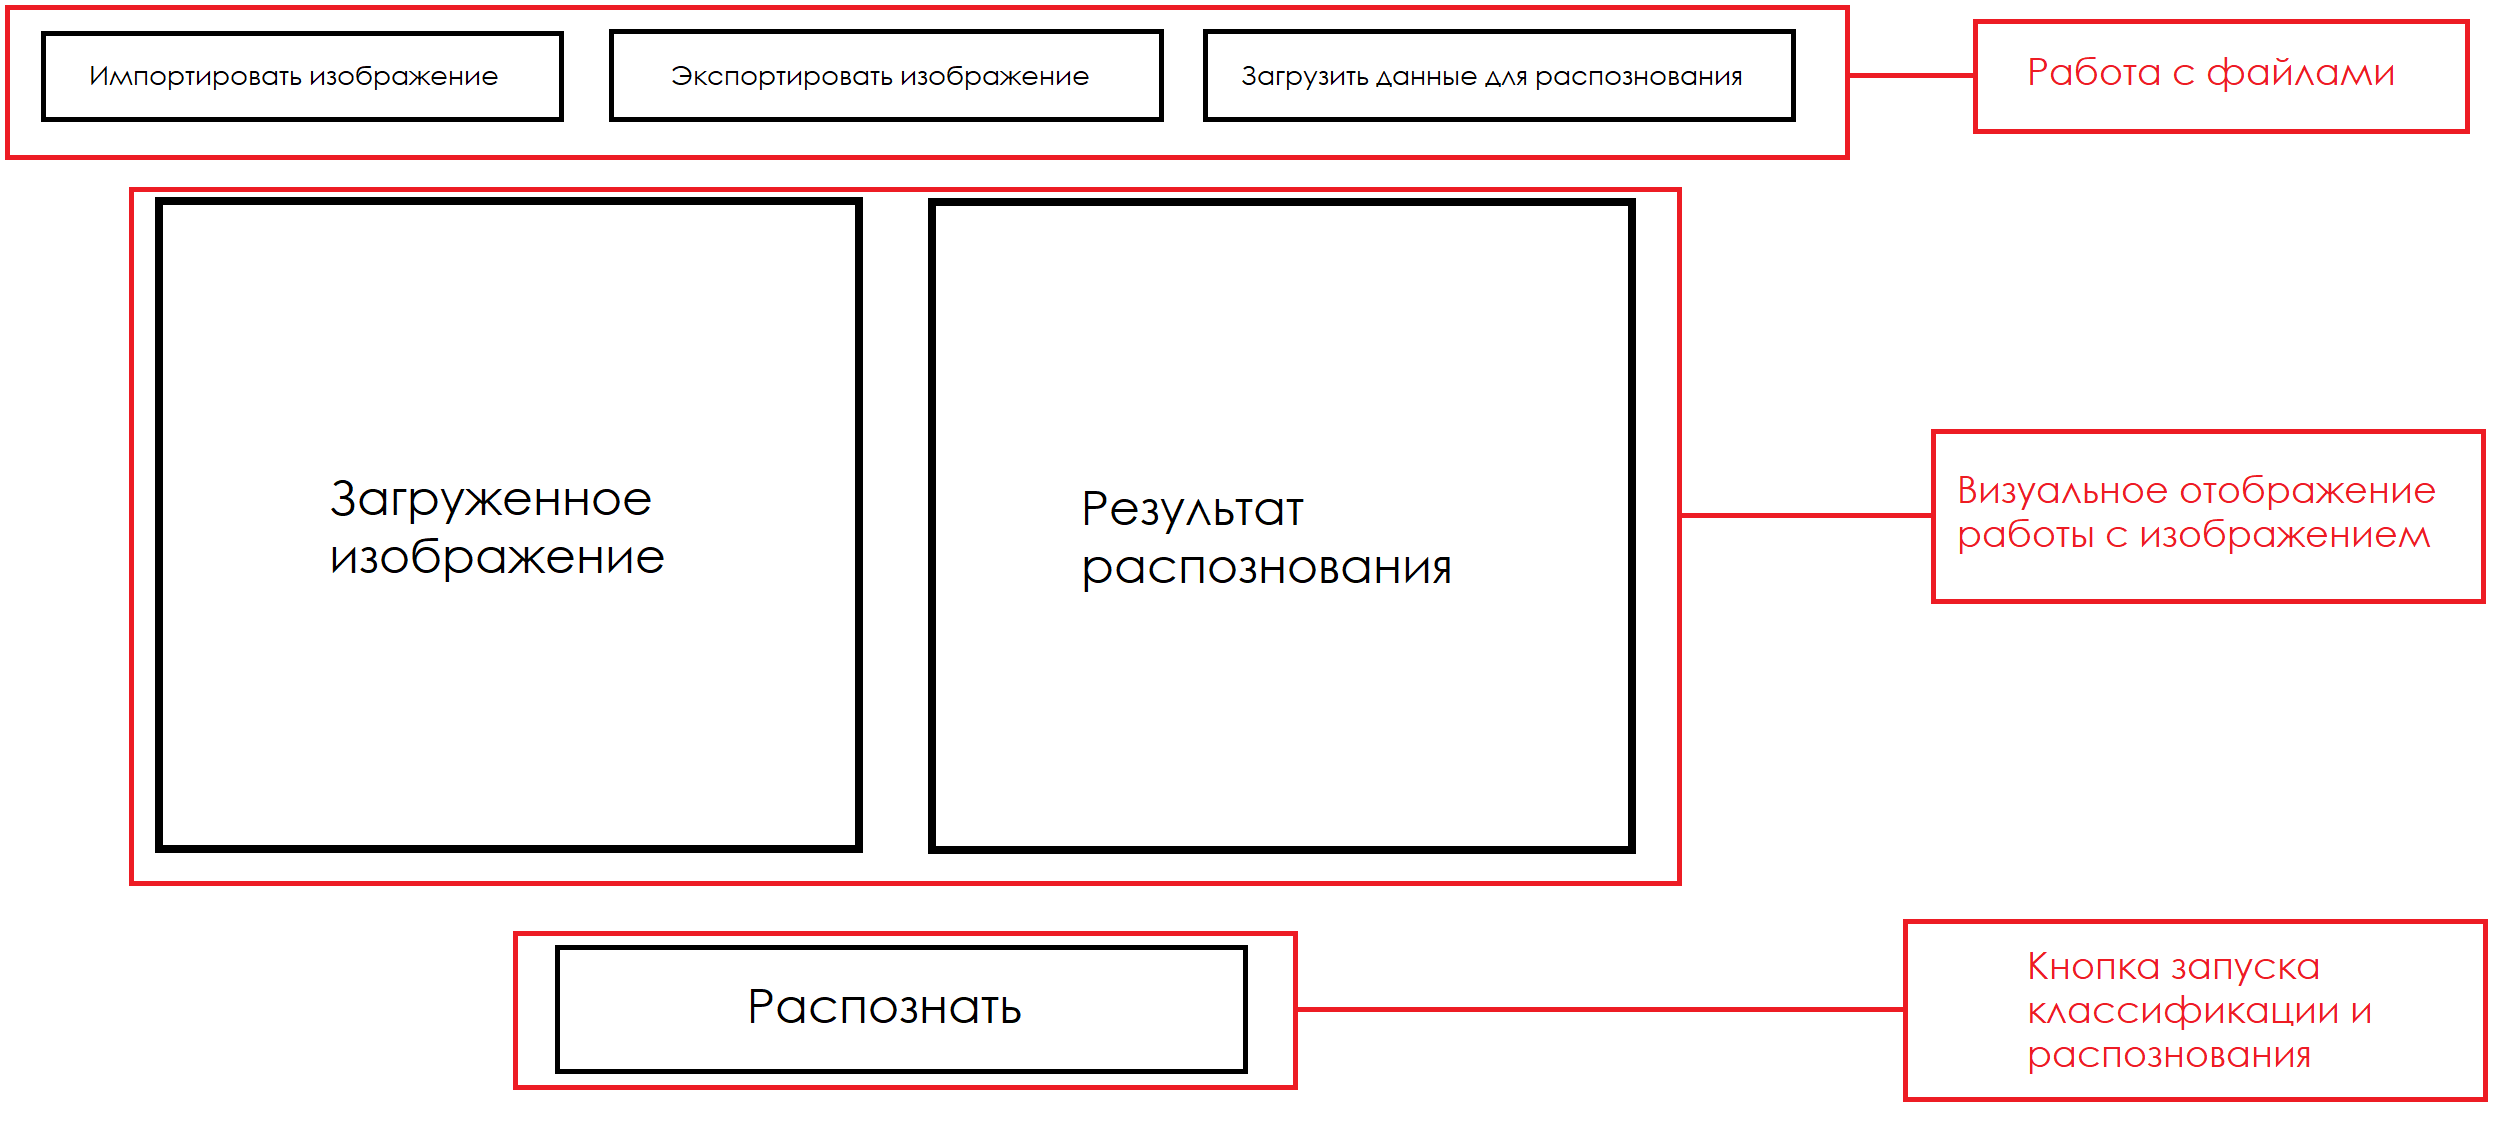
\includegraphics[width=1\linewidth]{shablon}
\caption{Композиция шаблона программы}
\label{shablon:image}
\end{figure}
%\vspace{-\figureaboveskip} % двойной отступ не нужен (можно использовать, если раздел заканчивается картинкой)
\subsection{Моделирование вариантов использования}

Для разрабатываемого сайта была реализована модель, которая обеспечивает наглядное представление вариантов использования приложения.

Она помогает в физической разработке и детальном анализе взаимосвязей объектов. При построении диаграммы вариантов использования применяется унифицированный язык визуального моделирования UML.

Диаграмма вариантов использования описывает функциональность разрабатываемой системы. Она отражает взаимодействие системы с актерами, такими как операторы БПЛА, службы реагирования и специалисты. Каждый прецедент на диаграмме описывает действия системы для актеров: загрузка изображения, загрузка данных для распознавания, само распознавание и вывод результирующего изображения. Диаграмма обеспечивает понимание целей системы, выявляя пробелы и соответствие потребностям заинтересованных сторон. Прецедент служит для описания набора действий, которые система предоставляет актеру.

Диаграмма предоставлена на рисунке ~\ref{actorusing:image}

\begin{figure}[ht]
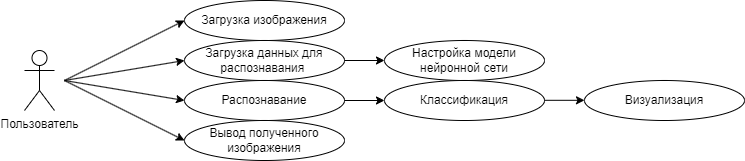
\includegraphics[width=1\linewidth]{actorusing}
\caption{Диаграмма вариантов использования}
\label{actorusing:image}
\end{figure}

\subsection{Требования к оформлению документации}

Разработка программной документации и программного изделия должна производиться согласно ГОСТ 19.102-77 и ГОСТ 34.601-90. Единая система программной документации.
